\documentclass[border=4pt]{standalone}
\usepackage{amsmath,amssymb,tikz}\usetikzlibrary{arrows.meta}
\definecolor{figB}{RGB}{31,90,166}\definecolor{figR}{RGB}{176,48,48}\definecolor{figG}{RGB}{46,125,50}\definecolor{figO}{RGB}{214,120,20}
\begin{document}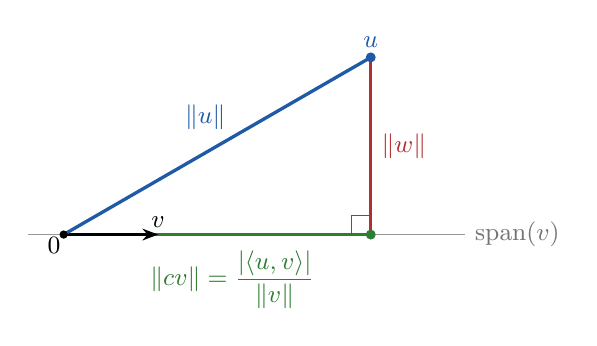
\begin{tikzpicture}[scale=1.5,>={Stealth[length=2mm]}]
\draw[black!40] (-0.3,0)--(3.4,0) node[right,font=\small,black!55]{$\operatorname{span}(v)$};
\draw[very thick,figG] (0,0)--(2.6,0) node[pos=0.55,below=2pt,font=\small]{$\|cv\|=\dfrac{|\langle u,v\rangle|}{\|v\|}$};
\draw[->,thick] (0,0)--(0.8,0) node[above,font=\small,inner sep=2pt]{$v$};
\draw[figR] (2.6,0.16)--(2.44,0.16)--(2.44,0);
\draw[very thick,figR] (2.6,0)--(2.6,1.5) node[midway,right,font=\small]{$\|w\|$};
\draw[very thick,figB] (0,0)--(2.6,1.5) node[pos=0.55,above left,font=\small,inner sep=2pt]{$\|u\|$};
\fill (0,0) circle (1pt) node[below left,font=\small,inner sep=1pt]{$0$};
\fill[figB] (2.6,1.5) circle (1.2pt) node[above,font=\small]{$u$};
\fill[figG] (2.6,0) circle (1.2pt);
\end{tikzpicture}\end{document}
